\documentclass[10pt,a4paper,twoside]{report}

% Just because this is useful
\newcommand{\mycomment}[1]{} %Multi-line comment

%Configuration document

%%%%%%%%%%%%%%%%%%%%%%%%%%%%%%%%%%%%%%%%%%%%%%%%%%%%%%%%%%%%%%%%%%%%%%%%%%%%%%%
% PACKAGES
%%%%%%%%%%%%%%%%%%%%%%%%%%%%%%%%%%%%%%%%%%%%%%%%%%%%%%%%%%%%%%%%%%%%%%%%%%%%%%%

%Language
\usepackage[utf8]{inputenc} 			% Input encoding
\usepackage[english]{babel} 			% English
\usepackage{csquotes}                   % ADDED to make sure quoted texts show up correctly.

%Mathematics
\usepackage{amsmath}					% American Mathematical Society Package
\usepackage{amsfonts}					% Mathematical Fonts
\usepackage{amssymb}					% More mathematical symbols
\usepackage{mathtools}					% More control and better appearance of Mathematics

%Figures and captions
\usepackage{graphicx}					% More complex version of graphics for figures
\usepackage[labelfont=bf,font=small]{caption}		% More control over captions (and boldface "Figure 1.1." text)
\usepackage[labelfont=bf,font=small]{subcaption}	% Same, for subcaptions
\usepackage{sidecap}					% Side captions (just in case)

\pdfsuppresswarningpagegroup=1			% This just suppresses an annoying (and meaningless) warning

%ThE LooOks!
\usepackage{fancyhdr}					% Fancy Headers
\usepackage{geometry}					% Control geometry
\usepackage{setspace}
\usepackage[bottom]{footmisc}           %Send footnotes to the bottom of the page

%Tables and other environments
\usepackage{tabularx}					% Better tables
\usepackage{booktabs}					% Even better tables
\usepackage{enumitem}					% More control over enumerate environments
\usepackage{arydshln}					% Use dashed lines in tables

%Physics
\usepackage{siunitx}					% SI units			
\usepackage{physics}					% Useful notations (bras and kets for example)

% Useful Tools
\usepackage{lipsum}						% Create random text
\usepackage{comment}					% Create comments
\usepackage{xcolor} 					% Colors
\usepackage[dvipsnames]{xcolor} 		% Better Colors
\usepackage{framed}						% Colored frames

%My packages
\usepackage{slashed}                    % Feynman notation for Dirac matrices, i.e. \slashed{}
\usepackage{nccmath}                    % More math stuff (\mfrac for medium sized fractions!)
\usepackage{bbold}                      % For \mathbb{1}
\usepackage{multirow}                   % multirows
\usepackage{booktabs}                   % nice tables, idk
\usepackage{environ}                    %\NewEnviron{}{}{} to define environments

%Load last
\usepackage{hyperref}					% Create hyperlinks


%%%%%%%%%%%%%%%%%%%%%%%%%%%%%%%%%%%%%%%%%%%%%%%%%%%%%%%%%%%%%%%%%%%%%%%%%%%%%%%
% DOCUMENT SETUP
%%%%%%%%%%%%%%%%%%%%%%%%%%%%%%%%%%%%%%%%%%%%%%%%%%%%%%%%%%%%%%%%%%%%%%%%%%%%%%%

%Paper Geometry
\geometry{
	paper=a4paper, 	% A4 Paper
	inner=2.5cm, 	% Inner margin
	outer=2.5cm, 	% Outer margin
	top=2.5cm, 		% Top margin
	bottom=2.5cm, 	% Bottom margin
}

%Line spacing
\setstretch{1.5}

% ---------------------------
% SELECT THE MATH FONT
% NOTE: Comment out all of them for the default computer modern 

%\usepackage{mathpazo}	% Loads Palatino for math use (serifed math font)
\usepackage{cmbright}	% Loads Computer Modern Bright (normal text font can be different)

% ---------------------------
% SELECT THE NORMAL TEXT FONT

%\newcommand{\fontnamestring}{phv}	% Helvetica
\newcommand{\fontnamestring}{cmbr}	% Computer Modern Bright

\renewcommand{\rmdefault}{\fontnamestring}
\renewcommand{\sfdefault}{\fontnamestring}

\def\FontLn{% 16 pt normal
	\usefont{T1}{\fontnamestring}{m}{n}\fontsize{16pt}{16pt}\selectfont}
\def\FontLb{% 16 pt bold
	\usefont{T1}{\fontnamestring}{b}{n}\fontsize{16pt}{16pt}\selectfont}
\def\FontMn{% 14 pt normal
	\usefont{T1}{\fontnamestring}{m}{n}\fontsize{14pt}{14pt}\selectfont}
\def\FontMb{% 14 pt bold
	\usefont{T1}{\fontnamestring}{b}{n}\fontsize{14pt}{14pt}\selectfont}
\def\FontSn{% 12 pt normal
	\usefont{T1}{\fontnamestring}{m}{n}\fontsize{12pt}{12pt}\selectfont}




%------------------------
%-------- MINE ----------
%------------------------
%No adjustment, all blank space is sent to the bottom of the page
\raggedbottom


%%%%%%%%%%%%%%%%%%%%%%%%%%%%%%%%%%%%%%%%%%%%%%%%%%%%%%%%%%%%%%%%%%%%%%
% NOTE: THESE COMMANDS (ALL THREE) MAKE SURE THE MATH MODE IS BIGGER
%		I DIDN'T USE THEM, BUT IT MAY VERY WELL LOOK NICER

%Change math mode size
%\DeclareMathSizes{<tfs>}{<ts>}{<ss>}{<sss>}
% <tfs> --- Surrounding text
% <ts>  --- Mathmode text
% <ss>  --- Subscript
% <sss> --- Subsubscript

%%%%%%%%%%%%%%%%%%%%%%%%%%%%%%%%%%%%%%%%%%%%%%%%%%%%%%%%%%%%%%%%%%%%%%

% UNCOMMENT THE FOLLOWING THREE LINES
%\DeclareMathSizes{9}{10}{8}{6}
%\DeclareMathSizes{10}{10}{8}{6}
%\DeclareMathSizes{11}{10}{8}{6}

%--------------------------
% Enabling \mathscr{} for pretty calligraphic fonts. :)

\makeatletter
\DeclareFontEncoding{LS1}{}{}
\DeclareFontEncoding{LS2}{}{\noaccents@}
\DeclareFontSubstitution{LS1}{stix}{m}{n}
\DeclareFontSubstitution{LS2}{stix}{m}{n}
\makeatother

\DeclareMathAlphabet\mathscr{LS1}{stixscr}{m}{n}
\SetMathAlphabet\mathscr{bold}{LS1}{stixscr}{b}{n}
%--------------------------


%--------------------------
% Small bold for CMBright

\DeclareFontFamily{OT1}{cmbr}{\hyphenchar\font45 }
\DeclareFontShape{OT1}{cmbr}{m}{n}{%
	<-9>cmbr8
	<9-10>cmbr9
	<10-17>cmbr10
	<17->cmbr17
}{}
\DeclareFontShape{OT1}{cmbr}{m}{sl}{%
	<-9>cmbrsl8
	<9-10>cmbrsl9
	<10-17>cmbrsl10
	<17->cmbrsl17
}{}
\DeclareFontShape{OT1}{cmbr}{m}{it}{%
	<->ssub*cmbr/m/sl
}{}
\DeclareFontShape{OT1}{cmbr}{b}{n}{%
	<->ssub*cmbr/bx/n
}{}
\DeclareFontShape{OT1}{cmbr}{bx}{n}{%
	<->cmbrbx10
}{}

%--------------------------




%------------------------
%------------------------


%Make tables align at the separator '.'
\usepackage{dcolumn}
\newcolumntype{d}{D{.}{.}{-1}}

%URL links setup
\colorlet{url-blue}{blue!70!black}

\hypersetup{
    %pdftitle            = {Thesis Title},
	pdfpagemode			= {UseOutlines}	,
	bookmarksopen		= true 			,
	bookmarksopenlevel	= 0				,
	hypertexnames		= false			,
	colorlinks			= true			, % Set to false to disable coloring links
	citecolor			= blue			, % The color of citations
	linkcolor			= blue			, % The color of references to document(sections, figures, etc)
	urlcolor			= url-blue		, % The color of hyperlinks (URLs)
	pdfstartview		= {FitV}			,
	breaklinks			= true,
	unicode								,
}

%Setup sidecaption aligned to top of figure and caption width
\sidecaptionvpos{figure}{t}
\captionsetup{width=.85\textwidth}
%\captionsetup{width=.95\textwidth}


%Set shaded color
\definecolor{shadecolor}{rgb}{0.8,0.8,0.8}

%%%%%%%%%%%%%%%%%%%%%%%%%%%%%%%%%%%%%%%%%%%%%%%%%%%%%%%%%%%%%%%%%%%%%%%%%%%%%%%
% COVER PAGE TOOLS
%%%%%%%%%%%%%%%%%%%%%%%%%%%%%%%%%%%%%%%%%%%%%%%%%%%%%%%%%%%%%%%%%%%%%%%%%%%%%%%

%new Latex variable names
\newcommand{\coverThesis}{@undefined} 
\newcommand{\coverSupervisors}{@undefined}
\newcommand{\coverExaminationCommittee}{@undefined}
\newcommand{\coverChairperson}{@undefined} 
\newcommand{\coverSupervisor}{@undefined} 
\newcommand{\coverMemberCommittee}{@undefined} 

\addto\captionsenglish{\renewcommand{\coverThesis}{Thesis to obtain the Master of Science Degree in}}
\addto\captionsenglish{\renewcommand{\coverSupervisors}{Supervisors}}
\addto\captionsenglish{\renewcommand{\coverExaminationCommittee}{Examination Committee}}
\addto\captionsenglish{\renewcommand{\coverChairperson}{Chairperson}}
\addto\captionsenglish{\renewcommand{\coverSupervisor}{Supervisor}}
\addto\captionsenglish{\renewcommand{\coverMemberCommittee}{Members of the Committee}}

%%%%%%%%%%%%%%%%%%%%%%%%%%%%%%%%%%%%%%%%%%%%%%%%%%%%%%%%%%%%%%%%%%%%%%%%%%%%%%%
% ACKNOWLEDGEMENT SECTION
%%%%%%%%%%%%%%%%%%%%%%%%%%%%%%%%%%%%%%%%%%%%%%%%%%%%%%%%%%%%%%%%%%%%%%%%%%%%%%%

% new LaTeX variable name
\newcommand{\acknowledgments}{@undefined} 
\addto\captionsenglish{\renewcommand{\acknowledgments}{Acknowledgements}}

%%%%%%%%%%%%%%%%%%%%%%%%%%%%%%%%%%%%%%%%%%%%%%%%%%%%%%%%%%%%%%%%%%%%%%%%%%%%%%%
% NOMENCLATURE AND GLOSSARY
%%%%%%%%%%%%%%%%%%%%%%%%%%%%%%%%%%%%%%%%%%%%%%%%%%%%%%%%%%%%%%%%%%%%%%%%%%%%%%%

%-----------------------
% If you want the nomenclature table (list of variables). NOT REQUIRED BY IST

\usepackage{nomencl}
\makenomenclature

% Group variables according to their symbol type
\RequirePackage{ifthen}

\renewcommand{\nomgroup}[1]{%
	\ifthenelse{	\equal{#1}{R}	}{	\item[\textbf{Roman symbols}]	}{%
	\ifthenelse{	\equal{#1}{G}	}{	\item[\textbf{Greek symbols}]	}{%
   	\ifthenelse{	\equal{#1}{S}	}{	\item[\textbf{Subscripts}]		}{%
  	\ifthenelse{	\equal{#1}{T}	}{	\item[\textbf{Superscripts}]	}{%   
  	}}}}}
    

%-----------------------
% For the list of Abbreviations (required by IST)

% 'nomain'         - Do not use main glossary.
% 'acronym'        - Prints the acronyms. Pairs with previous option.
% 'nogroupskip'    - Eliminate spacing between groups of acronyms starting with the same letter.
% 'nopostdot'      - Does not insert a '.' at the end of acronym description (user must input by default).
% 'nonumberlist'   - Suppresses the list of document locations for each entry.
% 'indexonlyfirst' - Only adds to '.acr' file when an abbreviation is included in text for the first time.
% NOTE: THIS LAST ONE IS ONLY RELEVANT IF ONE REFERENCES THE ACRONYMS IN-TEXT (BY USING \Gls, OR SOME SUCH THING)

\usepackage[nomain,acronym,nogroupskip,nopostdot,nonumberlist,indexonlyfirst]{glossaries}
\makeglossaries


%----------------------------------
%------------ COMMANDS ------------
%----------------------------------
%----------------------------------
%------------ COMMANDS ------------
%----------------------------------
%
% Here, you can neatly define all your auxilliary commands

%Packages
\RequirePackage[dvipsnames]{xcolor}
\RequirePackage{fancyvrb} %Fancy Verbatim (used with \Verb)


%Commands
\newcommand{\ac}[1]{\textcolor{MidnightBlue}{#1}} %Andre's comments.
\newcommand{\orange}[1]{\textcolor{Bittersweet}{#1}} %Orange comments.
\newcommand{\green}[1]{\textcolor{OliveGreen}{#1}} %Green comments.

\newcommand{\mycomment}[1]{} %Multi-line comment

\newcommand{\sub}[1]{_{#1}^{}} %Subscripts with proper height
\newcommand{\upp}[1]{_{}^{#1}} %Superscripts with proper height
\newcommand{\ind}[2]{^{#1}_{#2}} %Both

\newcommand{\expo}{{\rm e}} %exp
\newcommand{\im}{{\rm i}} %imaginary unit

\newcommand{\diff}{{\rm d}} %differential

%--------

%Slashed with subscript
\newcommand{\slashedsub}[2]{\slashed{#1}\sub{\hspace{-.05cm}#2}}


%definitions
%\newcommand\myeq{\mathrel{\stackrel{\makebox[0pt]{\mbox{\normalfont\tiny $\int $}}}{=}}}
\newcommand\mydef{
	\mathrel{\stackrel{\makebox[0pt]{\mbox{\normalfont\tiny \textrm{ def} }}}{=}}
}

\newcommand\equalenforce{
	\mathrel{\stackrel{\makebox[0pt]{\mbox{\normalfont\scriptsize \textrm{ !} }}}{=}}
}

%Setup the document title (file properties)
\hypersetup{%
pdftitle={Thesis Title},%
}


%-----------------------------------
%-----------------------------------
%-----------------------------------

\begin{document}


%%%%%%%%%%%%%%%%%%%%%%%%%%%%%%%%%%%%%%%%%%%%%%%%%%%%%%%%%%%%%%%%%%%%%%%%%%%%%%%
% FRONT MATTER
%%%%%%%%%%%%%%%%%%%%%%%%%%%%%%%%%%%%%%%%%%%%%%%%%%%%%%%%%%%%%%%%%%%%%%%%%%%%%%%

\pagestyle{plain}
\pagenumbering{roman}

% ----------------------------------------------------------------------
%  Cover , Dedication and Acknowledgements pages
% ----------------------------------------------------------------------

%Cover page

%%%%%%%%%%%%%%%%%%%%%%%%%%%%%%%%%%%%%%%%%%%%%%%%%%%%%%%%%%%%%%%%%%%%%%%%%%%%%%%
% COVER PAGE OF MASTER THESIS
%%%%%%%%%%%%%%%%%%%%%%%%%%%%%%%%%%%%%%%%%%%%%%%%%%%%%%%%%%%%%%%%%%%%%%%%%%%%%%%

\thispagestyle{empty}

%IST Logo

\includegraphics[viewport = 9.5cm 11cm 0cm 0cm ,scale = 0.29]{Thesis_Template/inputs/01_Cover_Page/IST_A_CMYK_POS}

\begin{center}


%----------------------------------
% Figure (Image or plot)
\vspace{.05\textheight}
\begin{center}
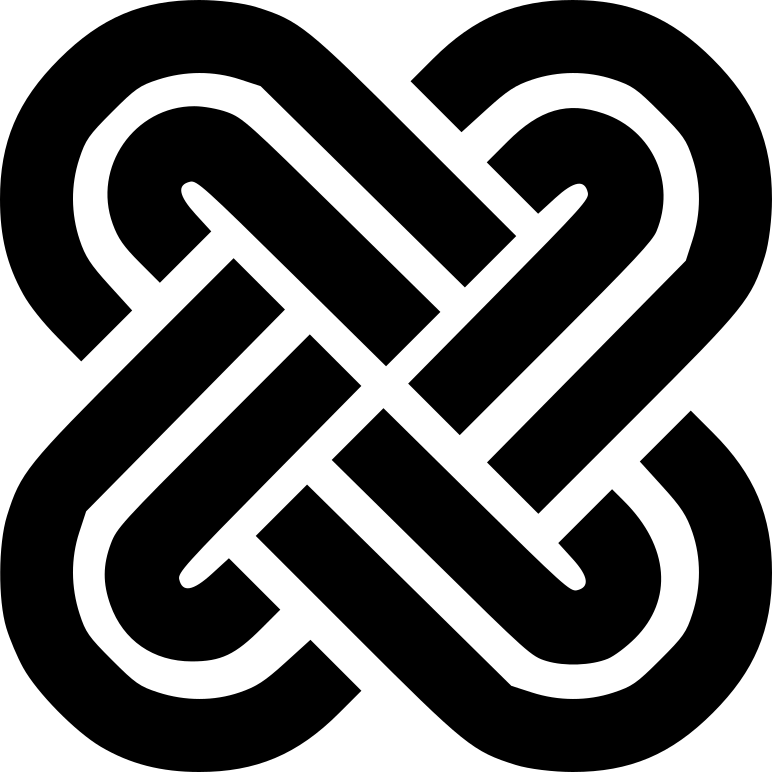
\includegraphics[height=.15\textheight]{Thesis_Template/inputs/01_Cover_Page/solomon}
\end{center}
\vspace{.025\textheight}

%Because I don't have a figure
%\vspace{.15\textheight}


%----------------------------------
% Thesis Title
\vspace{1.0cm}
{\FontLb [MSc Thesis Title]} \\ 
\vspace{0.2cm}
{\FontMn [MSc Thesis Subtitle]} \\
\vspace{0.9cm}

%Author name
\vspace{0.6cm}
{\FontMb [Author's Full Name]} \\ 

%Degree
\vspace{2.0cm}
{\FontSn \coverThesis} \\
\vspace{0.3cm}
{\FontLb [Degree Name]}  \\

%Supervisors
\vspace{1.0cm}
{\FontSn %
\begin{tabular}{ll}
	\coverSupervisors: & [Supervisor's Full Name] \\
	                   & [Co-Supervisor's Full Name]
\end{tabular} } \\

%Examination Commitee
\vspace{1.0cm}
{\FontMb \coverExaminationCommittee} \\
\vspace{0.3cm}
{\FontSn %
\begin{tabular}{rl}
	  \coverChairperson:    & [Chairperson's Full Name, as in Fénix]  \\
	  \coverSupervisor:     & [Supervisor's Full Name, as in Fénix]   \\
	Member of the Committee:	& [Committee Member's Full Name, as in Fénix] \\
								& [Committee Member's Full Name, as in Fénix]
\end{tabular} } \\

%Date of oral examination
\vspace{1.5cm}
{\FontMb [Month \& Year]} \\ 


\end{center}

\null\newpage
\null\newpage

%Dedication page

%%%%%%%%%%%%%%%%%%%%%%%%%%%%%%%%%%%%%%%%%%%%%%%%%%%%%%%%%%%%%%%%%%%%%%%%%%%%%%%
% DEDICATION PAGE
%%%%%%%%%%%%%%%%%%%%%%%%%%%%%%%%%%%%%%%%%%%%%%%%%%%%%%%%%%%%%%%%%%%%%%%%%%%%%%%

\null
\vskip5cm
\begin{flushright}
     You can use this space for a dedication\\
     Or maybe a quote
\end{flushright}
\vfill
\newpage
 
%\cleardoublepage
\null\newpage

%Acknowledgments page
\section*{\acknowledgments}

% Add entry in the table of contents as section
\addcontentsline{toc}{chapter}{\acknowledgments}

As a point of orthography, ``Acknowledgments'' is the American spelling, and ``Acknowledgements'' the other spelling. You can change the \verb|\acknowledgments| command in \texttt{thesis\_preamble.tex}.

This template is based on the one built by Diogo Ribeiro and Pedro Cosme. André Cordeiro later fixed some glitches with the formatting.


%
\vfill
%
{\centering % By centering this, it ends up *really* at the bottom of the page
\small{\it Here you can acknowledge a funding grant, or some organisation.}
}
%\cleardoublepage
\null\newpage

% ----------------------------------------------------------------------
%  %Abstract in mother language and English
% ----------------------------------------------------------------------

%Mother language
\section*{Resumo}

% Add entry in the table of contents as section
%\addcontentsline{toc}{section}{Resumo}
\addcontentsline{toc}{chapter}{Resumo}

\lipsum[1-2]

%
\vfill
%
{\centering %Adjust the numbers to taste
\begin{tabular}{p{0.25\linewidth} p{0.65\linewidth}}
	\textbf{\Large Palavras-chave:} & Palavra-Chave 1; Palavra-Chave 2; Palavra-Chave 3; \\%
									& Palavra-Chave 4; Palavra-Chave 5; Palavra-Chave 6    % 
\end{tabular}
}   
%\cleardoublepage
\null\newpage

%English
\section*{Abstract}

% Add entry in the table of contents as section
%\addcontentsline{toc}{section}{Abstract}
\addcontentsline{toc}{chapter}{Abstract}

\lipsum[1-2]

%
\vfill
%
{\centering %Adjust the numbers to taste
\begin{tabular}{p{0.25\linewidth} p{0.65\linewidth}}
	\textbf{\Large Keywords:} 	& Keyword 1; Keyword 2; Keyword 3 \\ %
								& Keyword 4; Keyword 5; Keyword 6    %
\end{tabular}
} 
%\cleardoublepage
\null\newpage


% ----------------------------------------------------------------------
%  Table of contents, list of tables, list of figures and nomenclature
% ----------------------------------------------------------------------

% NOTE: Change chapter -> section in \addcontentsline{toc}{<section/chapter>}
%		to determine whether is shows up as a chapter (bold) or a section (indented)

%Table of contents
\phantomsection
\renewcommand{\contentsname}{Table of Contents}
\addcontentsline{toc}{chapter}{\contentsname}
{\hypersetup{linkcolor=black}% Set these links to black
\tableofcontents%
}
\null\newpage
%\null\newpage

%List of tables
\phantomsection
%\addcontentsline{toc}{section}{\listtablename}
\addcontentsline{toc}{chapter}{\listtablename}
{\hypersetup{linkcolor=black}% Set these links to black
\listoftables%
}
\null\newpage
%\null\newpage

%List of figures
\phantomsection
\addcontentsline{toc}{chapter}{\listfigurename}
{\hypersetup{linkcolor=black}% Set these links to black
\listoffigures%
}
\null\newpage
%\null\newpage

% Nomenclature
\renewcommand{\nomname}{List of Symbols}
% In case you want to define your own nomenclature groups
\renewcommand{\nomgroup}[1]{%
	\ifthenelse{	\equal{#1}{R}	}{	\item[\textbf{Roman symbols}]	}{%
	\ifthenelse{	\equal{#1}{G}	}{	\item[\textbf{Greek symbols}]	}{%
	\ifthenelse{	\equal{#1}{S}	}{	\item[\textbf{Subscripts}]		}{%
	\ifthenelse{	\equal{#1}{T}	}{	\item[\textbf{Superscripts}]	}{%   
	\ifthenelse{	\equal{#1}{Z}	}{	\item[\textbf{Other}]			}{%
}}}}}}

% Separation between symbol and description
\setlength{\nomlabelwidth}{1.5cm}


% The definitions can be placed anywhere in the document body
% and their order is sorted by <symbol> automatically when
% calling makeindex in the makefile
%
% The \glossary command has the following syntax:
%
% \glossary{entry}
%
% The \nomenclature command has the following syntax:
%
% \nomenclature[<prefix>]{<symbol>}{<description>}
%
% where <prefix> is used for fine tuning the sort order,
% <symbol> is the symbol to be described, and <description> is
% the actual description.

% ----------------------------------------------------------------------
% Roman symbols [r]

\nomenclature[r]{$T\ind{a}{ij}$}{SU(N) generator.}

\nomenclature[r]{$f\ind{abc}{}$}{SU(N) structure functions.}

%Phantoms to force position (alphabetical)
\nomenclature[r]{$\phantom{}u(p)$}{Spinor for fermions (incoming).}
\nomenclature[r]{$\phantom{}\bar{u}(p)$}{Spinor for fermions (outgoing).}

\nomenclature[r]{$\phantom{}\bar{v}(p)$}{Spinor for antifermions (incoming).}
\nomenclature[r]{$\phantom{}v(p)$}{Spinor for antifermions (outgoing).}

\nomenclature[r]{$\mathscr{L}$}{Lagrangian, or lagrangian density.}
% ----------------------------------------------------------------------
% Greek symbols [g]

\nomenclature[g]{$\mu,\nu,\sigma$}{Spacetime indices.}

\nomenclature[g]{$\varepsilon\sub{\mu}(p)$}{Polarisation for gluons (incoming).}
\nomenclature[g]{$\varepsilon\sub{\mu}(p)\upp{*}$}{Polarisation for gluons (outgoing).}

\nomenclature[g]{$\gamma\upp{\mu}$}{Dirac matrix.}


% ----------------------------------------------------------------------
% Subscripts [s]

\nomenclature[s]{$i,j,k$}{Colour indices pertaining to the fundamental representation.}

% ----------------------------------------------------------------------
% Supercripts [t]

\nomenclature[t]{$a,b,c$}{Colour indices pertaining to the adjoint representation.}

% ----------------------------------------------------------------------
% Others

\nomenclature[z]{$\partial\sub{\mu}$}{Partial derivative.}


\phantomsection
\addcontentsline{toc}{chapter}{\nomname}
\printnomenclature
%\null\newpage

%Glossary
\renewcommand{\glossaryname}{List of Abbreviations}
%--------------------------------------------------------------------
% NOTE: CLEAR CACHE AND RECOMPILE AFTER EVERY CHANGE TO THIS FILE
%       THIS CAN BE DONE BY CLICKING IN THE 'LOGS AND OUTPUT FILES'
%       BUTTON, FOLLOWED BY THE "TRASHCAN"
%--------------------------------------------------------------------

% Example of a glossary instead of acronyms
% NOTE: TO PRINT THIS, CALL \printglossary
%\newglossaryentry{latex}
%{
%    name=\LaTeX,
%    description={Is a mark up language specially suited for scientific documents}
%}

%\newglossaryentry{lagrangian} %This is just a key, must not be capitalised (for some reason)
%{
%    name=Lagrangian,
%    description={Is a scalar function that determines the dynamics of some system}
%}

%NOTE: TO PRINT THIS, CALL \printglossary[type=\acronymtype, title=Acronyms]
%\newacronym{MEFT}{MEFT}{É Inclusivo!} 
%\newacronym{TEST}{TEST}{A Test for Overleaf. An addition} 
%
\newacronym{CERN}{CERN}{Conseil Européen pour la Recherche Nucléaire.} 
\newacronym{LHC}{LHC}{Large Hadron Collider.}
\newacronym{RHIC}{RHIC}{Relativistic Heavy Ion Collider.}
%
\newacronym{FF}{FF}{Fragmentation Function.} 
\newacronym{PDF}{PDF}{Parton Distribution Function.} 
%
\newacronym{QCD}{QCD}{Quantum Chromodynamics.} 
\newacronym{pQCD}{pQCD}{Perturbative Quantum Chromodynamics.} 
\newacronym{DLA}{DLA}{Double Logarithmic Approximation.} 
\newacronym{LLA}{LLA}{Leading Logarithmic Approximation.} 
\newacronym{DGLAP}{DGLAP}{Dokshitzer-Gribov-Lipatov-Altarelli-Parisi.}
\newacronym{C/A}{C/A}{Cambridge-Aachen.}
\newacronym{HIC}{HIC}{Heavy Ion Collision.}
\newacronym{QGP}{QGP}{Quark-Gluon Plasma.}
%
\newacronym{pp}{pp}{proton-proton.}
\newacronym{AA}{AA}{nucleus-nucleus.}
%
\newacronym{IQR}{IQR}{Interquartile Range.} 
% For correct hyperlink
\phantomsection
\addcontentsline{toc}{chapter}{\glossaryname}

\glsaddall
\printglossary[type=\acronymtype, title=\glossaryname]   %To print the acronyms

\null\newpage\null\newpage

%%%%%%%%%%%%%%%%%%%%%%%%%%%%%%%%%%%%%%%%%%%%%%%%%%%%%%%%%%%%%%%%%%%%%%%%%%%%%%%
% MAIN MATTER
%%%%%%%%%%%%%%%%%%%%%%%%%%%%%%%%%%%%%%%%%%%%%%%%%%%%%%%%%%%%%%%%%%%%%%%%%%%%%%%

\setcounter{page}{1}
\pagenumbering{arabic}

% ----------------------------------------------------------------------
%  Chapters
% ----------------------------------------------------------------------

\chapter{A Tour of the Template}
\label{chapter:template_tour}


This template is intended for use in Master's Theses at \textit{Instituto Superior Técnico}, and is in accordance with the guidelines in the \textit{Guia de Preparação da Dissertação 2015/16} (the most recent at time of writing). The current version is an adaptation of the templates developed and used by former MEFT students Pedro Cosme, Diogo Ribeiro, and André Cordeiro. André Cordeiro is responsible for the most recent changes to this version, especially with regards to the \textit{List of Symbols}, the disposition of the ``Sample Chapter'' \ref{chapter:SampleChapter}, and the configuration of the \textit{Bibliography} (mainly the hyperlinks).

The remainder of this chapter contains a description of the project structure, along with some noteworthy commands that may be edited to taste. Nonetheless, the user should read the configuration files (or \texttt{Ctrl + F} through them), in order to fine tune this template.


%----------------------------------
\section{Document structure}

This thesis template is separated into several files for easy editing. The \texttt{main.tex} file serves as the base document from where all other files are inserted. In the main folder you can find 4 separate folders.

\subsection{The {\normalfont\texttt{/config}} folder} %\normalfont to avoid a warning

The \texttt{/config} folder contains two configuration files that should be edited with care:
%
\begin{itemize}
\item \texttt{thesis\_preamble.tex} -- Contains all packages required by the template as well as some useful ones for writing mathematical expressions, defining tables and including figures. It also contains the commands for setting up the thesis geometry and looks.

\begin{itemize}
	\item \Verb*|\usepackage[labelfont=bf,font=small]{caption}| is used to set the ``\textbf{Figure X.Y:}'' to be in boldface. Same is done for subcaptions.
	\item \Verb*|\usepackage{cmbright}| and \Verb*|\newcommand{\fontnamestring}{cmbr}| are done to set the font to Computer Modern Bright for both math mode and normal text.
	\item \Verb*|\DeclareMathSizes{<tfs>}{<ts>}{<ss>}{<sss>}| is called to set the size of math mode, both in equations and inline. The arguments are respectively the size of surrounding text, the size for math mode, the size of subscripts, and the size of subsubscripts. It must be called twice, with \verb+<tfs>+ larger and smaller than the font size used in the document.
	\item \Verb*|\hypersetup| is called to set the options for hyperlinks inside the document (this includes e.g. the colour of references).
	\item \Verb*|\captionsetup{width=.85\textwidth}| is called to define the width of captions.
	\item \Verb*|\usepackage[<options>]{biblatex}| is called to configure the bibliography. Check these options carefully, reading the comments to each portion of the code.
\end{itemize}


\item \texttt{my\_commands.tex} -- Contains user defined commands. I have some packages used for this template, as well as some commands pertaining to typesetting subscripts and superscripts.
\end{itemize}

\subsection{The {\normalfont\texttt{/input}} folder} %\normalfont to avoid a warning

After the document is configured, the actual writing can begin. In the \texttt{/input} folder you will find several folders with several documents inside:

\begin{itemize}
\item \texttt{/01\_Cover\_Page} -- A cover according to \textit{IST} regulations. The names of the author, supervisors, and committee members must be added, as well as the name of the degree. You can also choose a cover image.

\item \texttt{/02\_Front\_Matter} -- The Front Matter of a thesis is composed of the \textit{Dedication}, \textit{Acknowledgements}, \textit{Abstract} and \textit{Resumo} files. In the \textit{Dedication} file you may dedicate the thesis to someone or write a quote. The \textit{Acknowledgements} page allow you to acknowledge a funding grant, some organisation, or people whose importance to you and your work should be mentioned. The \textit{Abstract} and \textit{Resumo} pages should be essentially the same (albeit in different languages) and should contain a brief summary of your work. Since the character limit is identical for both languages, it may be useful to have slightly different texts in the \textit{Abstract} and \textit{Resumo} chapters.

\item \texttt{/03\_Glossary\_and\_Nomenclature} -- The \textit{List of Abbreviations}/\textit{Glossary} pages should contain important acronyms that you use throughout the thesis. You may also include mathematical symbols to form a \textit{List of Symbols}/\textit{Nomenclature} page, although this is not mandatory. Special care must be taken when compiling these sections, as described below.

\item \texttt{/04\_Chapters} -- Most writing happens inside this folder. Here you should create a separate file for each chapter. Chapter files may start in the following manner

\begin{verbatim}
\chapter{Chapter name}
\label{chapter:chapter_name}
\end{verbatim}


\noindent as to allow you to refer to the chapter further down the writing.

\item \texttt{/05\_Appendix} -- The appendix folder works in the same fashion as the chapter folder. Separate files for each appendix should be created and edited.
\end{itemize}

\subsection{The {\normalfont\texttt{/figures}} folder} %\normalfont to avoid a warning
%
All graphics to be included in the main document should be placed inside this folder. We recommend separating the files to be included in separate folders according to the chapter they are to be placed in. The second chapter of this template contains some examples of how to incorporate the graphics in the main text.

\subsection{The {\normalfont\texttt{/bib}} folder} %\normalfont to avoid a warning

Finally, the bibliography is handled by the \texttt{/bib} folder. Inside you will find the bibliography file \texttt{my\_ref.bib} where all the references should be placed. The bibliography entries may have a format similar to:

\begin{verbatim}
@article{Einstein:1905,
author = {Einstein, Albert},
title = {On the electrodynamics of moving bodies},
doi = {10.1002/andp.200590006},
journal = {Annalen Phys.},
volume = {17},
year = {1905}
}
\end{verbatim}
%
and be cited with the \verb|\cite| command as \cite{Einstein:1905}. To cite multiple sources at once, do \cite{FeynCalc:1991,FeynCalc:2016,FeynCalc:2020}. To specify a page in a source, one can say \cite[p.~500]{Dokshitzer:1991} --- in fact, any text can be added after the reference, as \cite[Any text you might want]{Peskin:1995}.

The easiest way to assure consistency with the formatting of each entry is to retrieve them from the same website (\href{https://inspirehep.net/}{InspireHEP}, \href{https://ui.adsabs.harvard.edu/}{NASA/ADS}, ... ).

As a final note, in the \textit{Bibliography}, the title will also be an hyperlink to the URL, DOI, ISBN, or ISSN, \textbf{in that order of priority}. Therefore, if an article has an open-access version, include the URL in the \texttt{.bib} file, and it will be used for the hyperlink.

%----------------------------------
\section{Useful links}
%
To take the biggest advantage possible of this template it is useful to know the ins and outs of \LaTeX. This usually takes time, but it is not a daunting task. For a start, the \href{https://www.overleaf.com/learn}{Overleaf website} contains some straightforward tutorials on how to edit \LaTeX\, files. After the basics, \href{https://tex.stackexchange.com}{the \LaTeX\, stackexchange} can help you with more specific problems -- there is almost always someone with a similar problem!

%----------------------------------
\section{How to compile this template}

When making changes to the \textit{List of Abbreviations}, \textit{List of Symbols}, or the \textit{Bibliography}, one must recreate some auxiliary files in order for the changes to take effect.

\subsection{TeXstudio}

\noindent In \textit{TeXstudio}, this can be achieved by:
\begin{itemize}
	\item Altering the glossary;
	\item Compiling the \texttt{.tex} file [F5];
	\item Producing the glossary auxiliary files [F9];
	\item Compiling the \texttt{.tex} file \textbf{again} [F5].
\end{itemize}

\noindent Note, if the change involves erasing a line from the \textit{List of Abbreviations} (\textit{Glossary}), the last two steps may need to be repeated (keep producing the glossary files and recompiling the project). Besides the hotkeys, these commands can be found in the \textit{Tools} menu in the upper bar.

For the \textit{Bibliography}, a similar procedure is required. This is also true for the \textit{List of Symbols} (\textit{Nomenclature}), with an additional caveat that the compilation command in \textit{Options} $\rightarrow$ \textit{Configure TeXstudio} $\rightarrow$ \textit{Commands} $\rightarrow$ \textit{Make Index} should be changed to one of the following
\begin{verbatim}
	makeindex.exe %.nlo -s nomencl.ist -o %.nls
	makeindex %.nlo -s nomencl.ist -o %.nls
\end{verbatim}

\noindent on Windows and Linux systems respectively. The command to build the auxiliary files for the nomenclature can be found in \textit{Tools}, named \textit{Index} (you can define a hotkey in \textit{Configure TeXstudio}).

\subsection{Overleaf}

\noindent In \textit{Overleaf}, it is enough to delete the cached files before recompiling the project. This can be done by clicking the \textit{Logs and output files} button (which displays the compilation errors and warnings), followed by the \textit{Trash Can} icon. Note, this is not necessary when deleting or re-adding an element of the glossary, only when making changes.

This behaviour was verified on \textit{Overleaf}, with the \textit{pdfLaTeX} compiler, using TeX Live version 2020.



\null\newpage
%\null\newpage

\chapter{A Sample Chapter}
\label{chapter:SampleChapter}

This chapter contains some examples of equations, figures, and tables with a suggested style.

%\clearpage
\section{Some Equations}

\subsection{Font Size in Math Mode}

To change the font size of inline math, such as $\sqrt{x\upp{2} + 1}$, $f\sub{p/h}(x, Q\upp{2})$, or $\tau\ind{-1}{\sf form} \propto z \,\theta\upp{2}$, consider the following lines on the file \texttt{thesis\_preamble.tex},

\begin{figure}[h!]
\centering
\begin{BVerbatim}
	\DeclareMathSizes{9}{10}{8}{6}
	\DeclareMathSizes{10}{10}{8}{6}
	\DeclareMathSizes{11}{10}{8}{6}
\end{BVerbatim}
\end{figure}


\noindent where the arguments of \verb+\DeclareMathSizes{<tfs>}{<ts>}{<ss>}{<sss>}+ are respectively, the size of surrounding text, the size for math mode, the size of subscripts, and the size of subsubscripts.
%
This command should be called at least twice, with \verb+<tfs>+ larger and smaller than the font size used in the document. 

\subsection{Single Line, Single Label Equation}

\begin{align}
	\diff \ln \rho\upp{2} \, \diff z
	\,=\,
	{\rm det}
	\begin{bmatrix}
		\,1 & f'(z) / f(z) \\
		\,0 & 1
	\end{bmatrix} 
	\diff \ln \mu\upp{2} \, \diff z
	\,=\,
	\diff \ln \mu\upp{2} \, \diff z
	\,.
\end{align}

\subsection{Multiple Line, Single Label Equation}

\begin{align} \begin{split}
	\mathscr{L}\sub{\textsf{classical}} \,&=\, 
	\overline{\psi} ( \im \slashed{D} - {\sf M} ) \psi - \frac{1}{4} F\ind{a}{\mu\nu} F\ind{a,\mu\nu}{} \,,
	\quad\textrm{ with }\quad\\
	%%%%%%%%%%%%%%%%%%%%%%%%
	D\sub{\mu} \,&=\, \partial\sub{\mu} \,-\, \im\,g\, \textrm{T}\upp{a} \, A\ind{a}{\mu} \,,\\
	F\ind{a}{\mu\nu} \,&=\, \partial\sub{\mu} A\ind{a}{\nu} \,-\, \partial\sub{\nu} A\ind{a}{\mu}
	\,+\, g\, f\upp{abc}\,A\ind{b}{\mu}\,A\ind{c}{\nu}\,.
\end{split} \end{align}

\subsection{Multiple Line, Multiple Label Equation}

\begin{subequations} \begin{align}
		\mfrac{1}{(-g)} \mathcal{M}&\sub{\mathcal{B} \rightarrow q\overline{q}g }
		=
		\varepsilon\sub{\mu}(k)\upp{*} \,
		\overline{u}(p\sub{1})
		\textrm{T}\ind{a}{ij}
		\bigg(
		\gamma\upp{\mu}
		\frac{ \slashed{k} + \slashed{p}\sub{1} + m }{ (p\sub{1} + k)\upp{2} - m\upp{2} }
		\mathcal{B}
		\,-\,
		\mathcal{B}
		\frac{ \slashed{k} + \slashed{p}\sub{2} - m }{ (p\sub{2} + k)\upp{2} - m\upp{2} }
		\gamma\upp{\mu}
		\bigg)
		v(p\sub{2})
		\\
		%----------------------------------------
		=&\,
		\overline{u}(p\sub{1})
		\, \mathcal{B} \,
		v(p\sub{2}) \,
		\varepsilon\sub{\mu}(k)\upp{*} \,
		\bigg(
		\frac{ p\ind{\mu}{1} }{ p\sub{1}\cdot k }
		\,-\,
		\frac{ p\ind{\mu}{2} }{ p\sub{2}\cdot k }
		\bigg) \textrm{T}\ind{a}{ij}
		%----
		+ \overline{u}(p\sub{1})
		\bigg(
		\frac{ \slashed{\varepsilon}\upp{*} \, \slashed{k} \, \mathcal{B} }{ 2 \, p\sub{1}\cdot k }
		\,-\,
		\frac{ \mathcal{B} \, \slashed{k} \, \slashed{\varepsilon}\upp{*} }{ 2 \, p\sub{2}\cdot k }
		\bigg)
		v(p\sub{2})
		\textrm{T}\ind{a}{ij}
		\label{eqline:amplitude_antenna}
		\,.
\end{align} \label{eq:amplitude_antenna} 
\end{subequations}
%
Here we see equation \eqref{eq:amplitude_antenna}, with special emphasis on line \eqref{eqline:amplitude_antenna}.



%------------------------------

%\clearpage
\section{Some Figures}

\subsection{Single Figure}

\begin{figure}[!ht]
	\centering
	\includegraphics[width=.40\linewidth]{example-image-a}
	\caption{A figure, with a caption. A very long caption. A really rather long caption, to show off the line width for captions.}
	\label{fig1:single_image}
\end{figure}


%\clearpage
\subsection{Side By Side}

\begin{figure}[!ht]
	\centering
	\begin{subfigure}[t]{.40\textwidth}
		\centering
		\includegraphics[width=\linewidth]{example-image-a}
		\subcaption{A sub-figure.}
		\label{subfig1:left_subimage}
	\end{subfigure}
	\hspace{.10\textwidth} % some spacing. Alternatively, \hfill works well
	\begin{subfigure}[t]{.40\textwidth}
		\centering
		\includegraphics[width=\linewidth]{example-image-b}
		\subcaption{Another sub-figure.}
		\label{subfig1:right_subimage}
	\end{subfigure}
	\caption{Two different sub-figures.}
	\label{fig1:two_images}
\end{figure}

In \ref{fig1:two_images}, we have two images, \ref{subfig1:left_subimage} and \ref{subfig1:right_subimage}, side by side.

%\lipsum[4-5]

\clearpage
\subsection{Three Figures}

\begin{figure}[!ht]
	\begin{subfigure}[t]{.40\textwidth}
		\centering
		\includegraphics[width=\linewidth]{example-image-a}
		\subcaption{First.}
		\label{subfig1:first_image}
	\end{subfigure}
	\hspace{.10\textwidth}
	\begin{subfigure}[t]{.40\textwidth}
		\centering
		\includegraphics[width=\linewidth]{example-image-b}
		\subcaption{Second.}
		\label{subfig1:second_image}
	\end{subfigure}
	\centering
	\begin{subfigure}[t]{.40\textwidth}
		\centering
		\includegraphics[width=\linewidth]{example-image-c}
		\subcaption{Third.}
		\label{subfig1:third_image}
	\end{subfigure}
	\caption{Three sub-figures, in the same image.}
	\label{fig1:three_images}
\end{figure}

%\clearpage
\section{Some Tables}

\subsection{A Simple Table}

\begin{table}[ht!]
	\centering
	\begin{tabular}{c c c c c c c}
		\toprule
		\textbf{Measurement} & 
		$1$ & 	$2$ & 	$3$ & 	$4$ & 	$5$ & $6$ 
		\\
		%------------------------------
		\midrule
		Experiment 1 
		& \num{4.20}	
		& \num{27.13}	
		& \num{70.06}	
		& \num{133.35}	
		& \num{180.42}	
		& \num{267.73}	\\ 
		Experiment 2 
		& \num{6.34}	
		& \num{37.72}	
		& \num{99.00}	
		& \num{132.12}	
		& \num{201.62}	
		& \num{221.37}	\\ 
		Experiment 3 
		& \num{10.62}	
		& \num{64.53}	
		& \num{171.98}	
		& \num{282.91}	
		& \num{335.09}	
		& \num{541.63}  \\
		\bottomrule
	\end{tabular}
	\caption{Table with a simple structure.}
	\label{tab4:tauform_vals}
\end{table}



\subsection{A More Complicated Table}

\begin{table}[ht]
	\centering
	\begin{tabular}{c c c c c}
		\toprule
		\multirow{2}{*}{\textbf{Analysis Methods}} &
		\multicolumn{4}{c}{\textbf{Data Sets}} \\
		%------------------------------
		& 
		\textbf{Data Set 1} & 
		\textbf{Data Set 2} & 
		\textbf{Data Set 3} & 
		\textbf{Data Set 4} \\
		%------------------------------
		\midrule
		Method 1	& \num{5.09}	& \num{4.15}	& \num{6.02}	& \num{8.49}		\\ 
		Method 2	& \num{2.19}	& \num{2.09}	& \num{4.44}	& \num{4.74}		\\ 
		\bottomrule
	\end{tabular}
	\caption{Table with a somewhat less simple structure.}
	\label{tab2:tau_form_resolution_mean}
\end{table}

\null\newpage
%\null\newpage




% ----------------------------------------------------------------------
%  Bibliography
% ----------------------------------------------------------------------

\phantomsection
\addcontentsline{toc}{chapter}{\bibname}

%\nocite{*}

\printbibliography
\null\newpage\null\newpage

%%%%%%%%%%%%%%%%%%%%%%%%%%%%%%%%%%%%%%%%%%%%%%%%%%%%%%%%%%%%%%%%%%%%%%%%%%%%%%%
% AFTER MATTER
%%%%%%%%%%%%%%%%%%%%%%%%%%%%%%%%%%%%%%%%%%%%%%%%%%%%%%%%%%%%%%%%%%%%%%%%%%%%%%%
\appendix

\chapter{An Appendix}
\label{appendix:app_name}


\lipsum[1-3]
\null\newpage
\null\newpage


\end{document}